\newpage
\noindent
\textbf{Beispiel 3}\\ \\
a)\\ \\
Freigeschnittene Körper:
\begin{figure}[h]
	\centering
	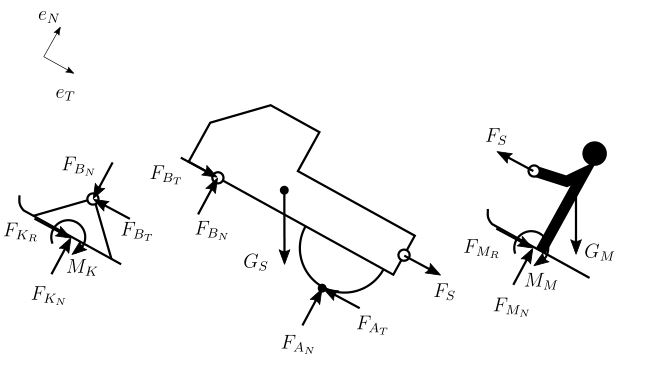
\includegraphics[width= 10cm]{tikz/01_02_2019_3a}
\end{figure}
b)\\ \\ 
Die Gleichgewichtsbedingungen für den Skifahrer lauten
\begin{align*}
	\textbf{e}_N &: F_{M_N} - G_M\cos(\alpha) = 0\\
	\textbf{e}_T &: F_{M_R} - F_S + G_M\sin(\alpha) = 0
\end{align*}
Durch miteinbeziehen der trockenen Gleitreibung folgt aus den beiden Gleichungen die Seilkraft
\[
	F_S = G_M(\mu_G\cos(\alpha) + \sin(\alpha))
\]
c)\\ \\
Die Gleichgewichtsbedingungen für die Kufe lauten
\begin{align*}
	\textbf{e}_N &: F_{K_N} - F_{B_N} = 0\\
	\textbf{e}_T &: F_{K_R} - F_{B_T} = 0
\end{align*}
Aus diesen Gleichung ergibt sich für die trockene Gleitreibung unter der Kufe
\[
	F_{B_T} = \mu_G F_{B_N}
\]
d)\\ \\
Die Gleichgewichtsbedingungen für das Schneemobil lauten
\begin{align*}
	\textbf{e}_x &: F_{B_T} - F_{A_T} + F_S + G_S\sin(\alpha) = 0\\
	\textbf{e}_y &: F_{B_N} + F_{A_N} - G_S\cos(\alpha) = 0\\
	\textbf{e}_z &: -F_Sh_M - G_S\sin(\alpha)h_S + G_S\cos(\alpha)l_S - F_{B_N}l_{AB} - F_{B_T}h_B = 0
\end{align*}
\newpage
\noindent
Aus diesen Gleichung folgen für sämtliche Lagerkräfte
\begin{align*}
	F_{B_N} &= \frac{G_Sl_S\cos(\alpha) - G_Sh_S\sin(\alpha) - F_Sh_M}{l_{AB} + \mu_Gh_B} \\
	F_{B_T} &= \mu_GF_{B_N} \\
	F_{A_N} &= G_S\cos(\alpha) - F_{B_N} \\
	F_{A_T} &= F_{B_T} + F_S + G_S\sin(\alpha)
\end{align*}
e)\\ \\
Die Haftbedingung lautet für den Punkt A
\[
	F_{A_T} \leq \mu_H F_{A_N}
\]
f)\\ \\
Damit das Schneenmobil nicht kippt muss die Bedingung
\[
	G_Sl_S\cos(\alpha) \geq G_Sh_S\sin(\alpha) + F_Sh_M + F_{B_N}(l_{AB} + \mu_Gh_B)
\]
erfüllt sein.\\ \\
